\section{Graphical building block diagram}
In this section, we show a graphical diagram representing the architecture of our system, which will be explained in detail in the following section.

\begin{figure}[H]
    \centering
    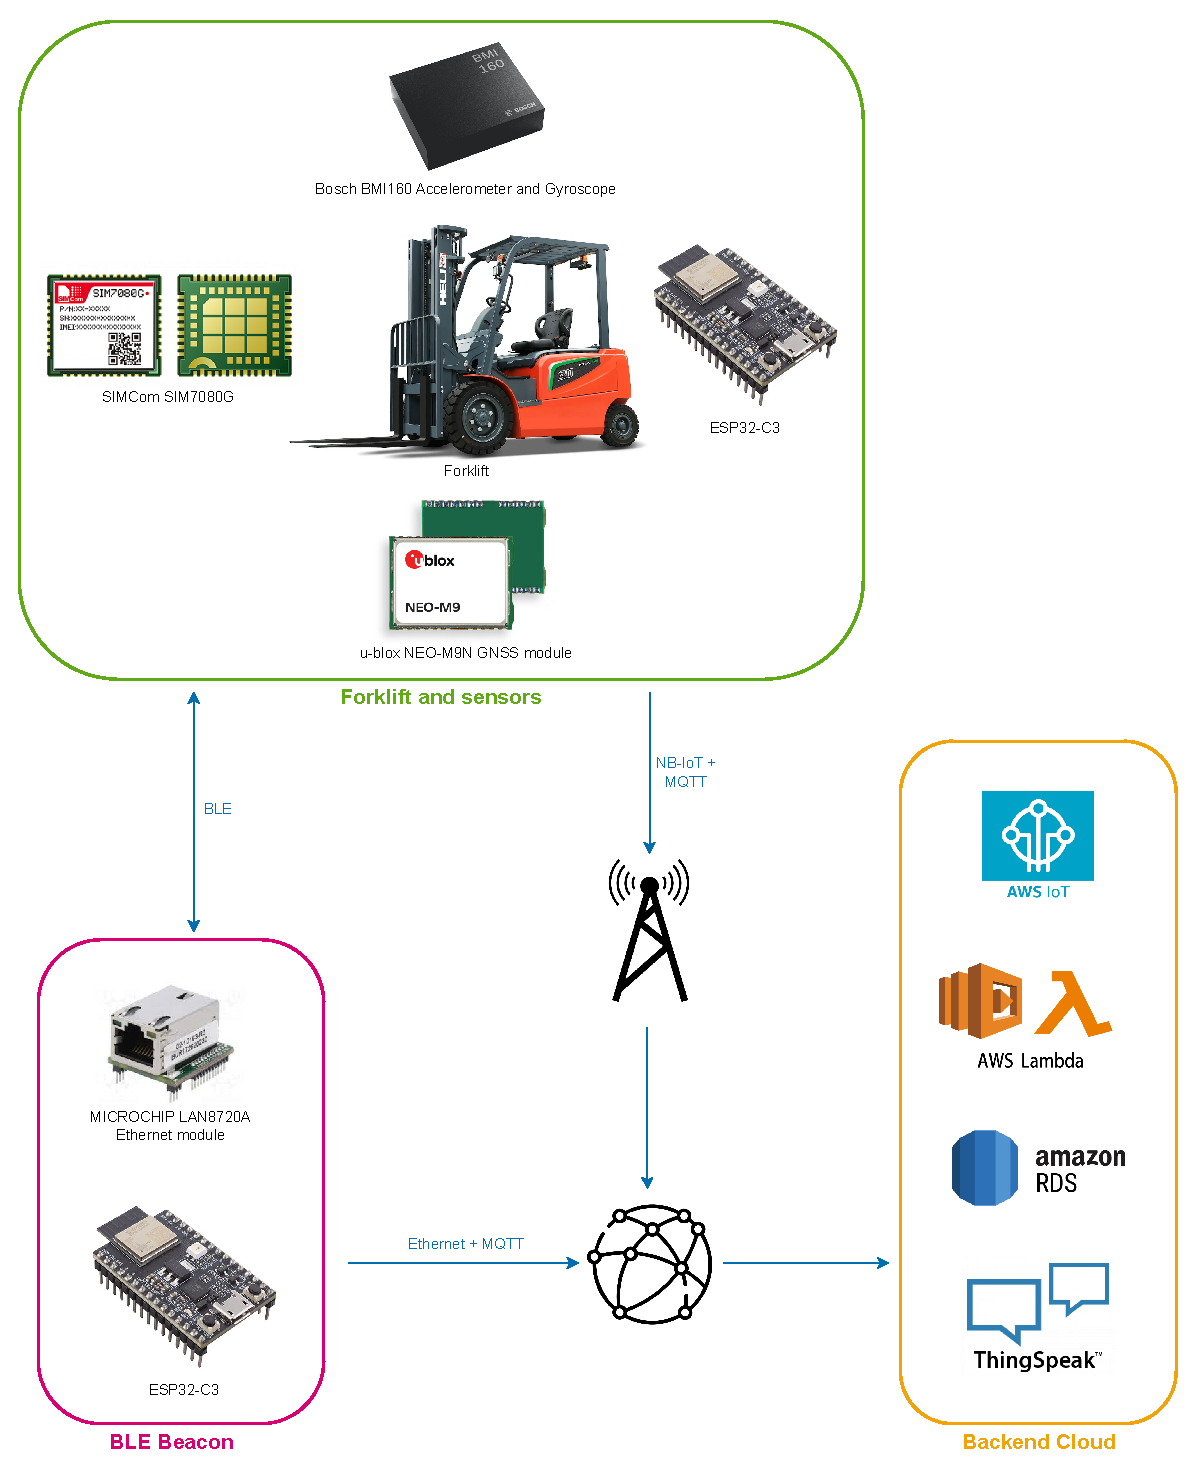
\includegraphics[width=\linewidth, height=0.6\textheight, keepaspectratio]{diagram.pdf}
    \caption{Graphical building block diagram}
\end{figure}

\section{Hardware and sensors}
Every forklift is equipped with an ESP32-C3 board, which natively supports BLE, and a SIMCom SIM7080G module enabling NB-IoT connectivity. Moreover, every forklift has a set of sensors which are used for different purposes:
\begin{itemize}
\item \textbf{Bosch BMI160 Accelerometer and Gyroscope}\\
Every forklift is equipped with two compact and low power sensors. One sensor is placed on a forklift’s wheel and is used as a gyroscope to measures the speed of the vehicle. The second sensor is placed on a non-moving part of the forklift and is used to measure its acceleration to perform impact detection; the sensor is set so that, when it measures a very high acceleration value (bigger than a threshold), the sensor wakes the ESP32-C3 with an interrupt.
\item \textbf{u-blox NEO-M9N GNSS module}\\
Every forklift also features a GPS module, used to track its position in the outdoor yard of the warehouse, providing an accuracy of about 1.5 meters.
\end{itemize}

Additional hardware is installed in the warehouse to localize forklifts:
\begin{itemize}
\item \textbf{ESP32-C3 boards (BLE beacons)}\\
In the internal area of the warehouse, we place nine ESP32-C3 boards, forming a reticule, so that there is a distance of 10 to 15 meters between them. These boards are used as BLE beacons to localize the forklifts. Forklifts exchange packets with these beacons and perform triangulation to compute their position in the warehouse.
\item \textbf{MICROCHIP LAN8720A Ethernet module}\\
ESP32-C3 boards used as BLE beacons are connected to the power supply and to the wired Internet of the warehouse, through an Ethernet module.
\end{itemize}
We assume that the internal area of the warehouse already features power supply and a stable wired Internet connection, which is used by the company.

\section{Communication protocols}
The system uses different communication protocols for indoor and outdoor areas of the warehouse, since they different in size by a large factor: the internal area is 500 $m^2$, while the external one is 1 $km^2$, i.e. 1 million $m^2$.\\
When they are in the external yard, forklifts communicate to the backend through NB-IoT, a long range technology that allows IoT devices to communicate at long distances and with low power consumption. We chose NB-IoT over LoRaWAN, another long range technology, because it is more suitable for a real time application, like the one we are implementing. Since the system needs to monitor forklifts in real time, vehicles need to communicate a new message every few seconds; LoRaWAN imposes a duty cycle of 1\% in Europe, has a low transmission rate and would probably suffer from collisions. NB-IoT, instead, requires a network plan with an ISP and network coverage from the provider, but has a higher transmission rate, allowing forklifts to communicate frequently their data to the backend. Finally, NB-IoT is very simple to use and has lower initial investment costs, since the infrastructure is provided by the ISP.\\
When forklifts are in the internal area of the warehouse, NB-IoT connectivity might not be sufficiently strong; that’s why forklifts in the underground area can communicate using BLE. This technology can be used both to localize forklifts in the underground warehouse and to allow them to send periodic information and impact information to the backend; we chose it because it is low cost and provides low range, which is needed for the underground area. Since the communication is unidirectional, the ESP32-C3 mounted on every forklift uses BLE in Advertising mode to broadcast packets to BLE beacons, which are mounted on the ceiling of the warehouse. Every message can reach multiple beacons, which ensures redundancy; beacons forward the message to the backend, which will discard copies of the same message, which can be identified by an ID contained in the payload of the message.\\
Both when using NB-IoT and BLE, packets are eventually sent to the backend using MQTT. When using NB-IoT, forklifts use TCP as Transport Layer and MQTT as Application Layer. While, when using BLE, BLE receivers process Advertising packets coming from forklifts, extract the payload, and translate them into MQTT messages, which are then forwarded over TCP and MQTT to backend, using the wired Ethernet connection.
Messages are published on two different topics:
\begin{itemize}
\item \verb|warehouse/<forkliftID>/impact|: topic used to publish impact detection messages, containing messageID, forkliftID, timestamp and position.
\item \verb|warehouse/<forkliftID>/status|: topic used to publish regular data about the status of the forklifts, containing messageID, forkliftID, timestamp, speed and position.
The forklift doesn’t send information about the travelled space, because it can be computed in the backend considering the value of speed and the time between one update and the following one.
\end{itemize}

\section{Status monitoring}
Forklift real time localization is performed using different technologies for the indoor and outdoor spaces. In the outdoor yard of the warehouse, forklifts use the NEO-M9N GNSS module to perform localization; this method combines an accuracy of about 1.5 to 2 meters, ideal for a large and open area, and low cost, making it an ideal choice for our system. In the indoor area of the warehouse, instead, forklifts are localized thanks to BLE RSSI, which is very low cost, reuses BLE beacons employed for communication and provides a reasonable accuracy of about 5 meters. Given the layout of the warehouse, we favoured using a simple and low cost solution, over a more precise and expensive one, such as UWB. BLE beacons periodically transmit packets containing a beacon identifier and the transmission power, forklifts who need to compute their position perform a BLE scan of 200 ms and receive Advertising packets from the beacons. Once the forklift has collected packets, it computes the distance from every beacon from which it received a packet using the log-distance path loss model. Finally, knowing the distance from beacons, the forklift identifies its position by triangulation with least-squares, and converts the obtained relative coordinates to absolute one, used also by GPS. The ESP32-C3 on the forklift checks if the GPS signal is strong enough, if it is, the forklift is in the outdoor yard, otherwise, the ESP-32 uses the BLE triangulation.\\ 
The system also monitors the speed and travelled distance by the forklifts, this is achieved by the ESP32-C3 thanks to BMI160 Gyroscope placed on a wheel of the forklift. Distance is computed by the backend, based on speed and the time elapsed between two following measurements. Position and speed data is sent from the ESP32-C3 to the backend every 5 seconds to guarantee real-time monitoring.

\section{Impact detection}
Impact detection is performed thanks to the Bosch BMI160 Accelerometer and Gyroscope mounted on the forklift. The sensor can be programmed to perform periodic measurements and send an interrupt to the ESP32-C3 on the forklift whenever the measured acceleration exceeds a threshold. When the board receives an interrupt, it notifies the backend. In order to detect the impact, we must choose an ODR that is fast enough to measure the high acceleration.  If we consider an impact acceleration of 5g, which is about 50 $m/s^2$, and a low  speed (worst case for the calculation) for the forklift of 10 km/h, the time it takes the forklift to stop is about 50 ms.

\begin{equation}
v = 50 \text{ km/h} = 2.78 m/s
\end{equation}

\begin{equation}
t = \frac{v}{a} = \frac{2.78 m/s}{50 m/s^2} = 55.6 ms
\end{equation}

We can use an ODR of 200 Hz, used by many impact detection applications, corresponding to measurements performed every 5 ms, a small enough time interval to be sure to measure the high acceleration value.

\section{Backend architecture}
The backend of the system is realized in cloud, using AWS IoT Core, a cloud service which can be used as a scalable MQTT broker that allows hosting in the cloud applications that process data generated by IoT devices. We process data using AWS Lambda and use Amazon RDS for PostgreSQL to store data in a relational database.\\
Every time the MQTT broker receives a message, a Python function in AWS Lambda processes the message, validates it, checks if it is a duplicate by checking if it already received a message with the same identifier. The function also publishes the received data to ThingSpeak, so that it can easily be accessed through a User Interface. Finally, the received data is stored in the database, offered by Amazon RDS.


\pagebreak
\section{Forklift Pseudocode}
\begin{minted}{cpp}

#define FORKLIFT_ID "1" //unique FORKLIFT_ID 
#define ACC_THRESHOLD 49.05 //5 * 9.81 m/s^2, 5g
#define GPS_HDOP_THRESHOLD 2.5 //gps precision threshold 
#define WHEEL_RADIUS 0.2  // wheel radius in meters
#define STATUS_INTERVAL 5000 //delay of 5s between two status measurments
struct Position {
    double lat;
    double long;
    bool valid;
};
struct Ble_packet {
    String beaconID;
    int rssi; //RSSI value
    Coord beacon_position; //local position of the beacon
};
void setup() {
    setup_gps();
    setup_accelerometer();
    setup_gyroscope();
    setup_ble_scan();
    last_status_time = now();
    nbiot_connect()
    setup_mqtt_client();
}

\end{minted}
\pagebreak
\begin{minted}{cpp}

void loop() {
    current_time = now();
    // impact detection measurment
    accel = read_accelerometer(vehicle)
    acc_magnitude = sqrt(accel.x² + accel.y² + (accel.z - 9.81)²)
    if (acc_magnitude > ACC_THRESHOLD) {
        // an impact has been detected
        position = get_position()
        impact_message = {
                "messageID": generate_uuid(),
                "forkliftID": forkliftID,
                "timestamp": current_time,
                "position": { "lat": position.lat, "lng": position.lng }
            }
        publish_message("warehouse/" + FORKLIFT_ID + "/impact", impact_message)
    }

    //perform status measurments each 5 seconds
    if (current_time - last_status_time >= STATUS_INTERVAL) { 
        //status measurments
        last_status_time = current_time
        position = get_position()
        gyro = read_gyroscope(wheel)
        //compute speed
        speed = gyro.z * wheel_radius
        status_message = {
                "messageID": generate_uuid(),
                "forkliftID": forkliftID,
                "timestamp": current_time,
                "speed": speed,
                "position": { "lat": position.lat, "lng": position.lng }
            }
        publish_message("warehouse/" + FORKLIFT_ID + "/status", status_message)
        }
    delay(500); //loop with ODR of 2Hz
}
\end{minted}

\begin{minted}{cpp}
void publish_message(String topic, Message message) {
    //check how the message should be sent
    payload = serialize_to_json(message);
    position = get_gps_position();
    if (!position.valid || position.hdop <= GPS_HDOP_THRESHOLD) {
        //forklift is inside => message published to BLE beacon
        String ble_payload = build_json_payload(topic, payload);
        //send message to all ble beacons
        ble_advertise(ble_payload);
    } else {
        //use nb-IoT
        mqtt_publish(topic, payload)
    }
}
Position get_position() {
    position = get_gps_position();
    if (!position.valid || position.hdop <= GPS_HDOP_THRESHOLD) {
        //forklift is inside => position retrieved through BLE
        ble_packets = perform_ble_scan(200); //200 is the scan duration in ms
        //ble_packets is an array of Ble_packet
        if (ble_packets.size >= 3) {
            beacons_position = [];
            distances = [];
            for pkt in ble_packet {
                beacons_position.append(pkt.beacon_position);
                //distance estimation using log-distance model
                dist = estimate_distance_rssi(pkt.rssi);
                distances.append(dist);
            }
            //retrieve local coordinates
            local_coord = least_squares_trialateration(beacons_position, distances);
            //convert local coordinates into absolute coordinates
            absolute_coord = local_to_absolute(local_coord.x, local_coord.y);
            return {
                lat: absolute_coord.lat,
                long: absolute_coord.long,
                valid: true
            }
        } else {
            //insufficient number of data
            return {lat: 0.0, long: 0.0, valid: false }
        }

    } else {
        //return gps position
        return position;
    }
}
\end{minted}
